%%%%%%%%%%%%%%%%%%%%%%%%%%%%%%%%%%%%%%%%%%%%%%%%%%%%%%%%%%%%%%%%%%%%%%%%%%%%%%%%%%%%%%%%%%%%%%%%%%%%%%%%%%%%%%%%%%%%%%%%%%%%%%%%%%%%%%%%%%%%%%%%%%%%%%%%%%%%%%%%%%%%%%%%%%%%%%%%%%%%%%%%%%%%%%%%%%%%%%%%%%%%%%%%%%%%%%%%%%%%%%%%%%%
\chapter{The Standard Model of particle physics}

%With the formulation of a relativistic quantum field theory and of spontaneous supersymmetry breaking by the Higgs mechanism, it was made possible to explain almost all observations of particle physics up to today.
The formulation of a relativistic quantum field theory and of spontaneous symmetry breaking (SSB) by the Brout-Englert-Higgs mechanism, allowed to built a theory which is capable to explain almost all observations of particle physics until today~\cite{bib:Theory:GFitter}.
This theory is known as the Standard Model of particle physics (SM).
The existence of its last missing piece, the Higgs boson, could be proven at the LHC in the year 2012~\cite{bib:Theory:CMS:HiggsObservation,bib:Theory:Atlas:HiggsObservation}.

The Standard Model is a $SU(3)_C  \times SU(2)_L \times SU(1)_Y$ non-abelian gauge theory.
``After'' spontaneous symmetry breaking, its symmetries are reduced to $SU(3)_C \times U(1)_{EM}$.
All particles that were found until today are contained in it\footnote{One can argue, that the right-handed neutrino, which is proven to exist, is not contained. But as at least the left-handed neutrino is embedded, we want to ignore that for a moment.}.
Furthermore, it is able to describe three of the four fundamental forces: the strong, weak and electromagnetic force.

In the following, a small introduction to the theory and phenomenology of the Standard Model is given.
It is not meant as a complete description.
The reader is referred to~\cite{bib:SM_book_Peskin,bib:SM_book_Ryder,bib:SM_book_Griffiths}, for a thorough and extensive introduction.

\section{The particle content}
It should be first noted, since the Standard Model is a quantum field theory, every field (to be more precise every degree of freedom of a field) can be considered also as a particle and vice versa.

The Standard Model of particle physics contains three different particle types, or three different types of fields.
First, there are the so-called ``matter particles'', which are all spin\,1/2 particles in the SM.
Second, the forces are described by spin\,1 vector bosons.
And finally, in order to give masses to all particles the Standard Model embeds the Higgs boson, a scalar spin\,0 particle.

\subsection*{Fermions in the Standard Model}
The fermionic content can be further subdivided into leptons and quarks.
In contrast to quarks, leptons are not strongly interacting, thus they only couple electromagnetically and weakly to other particles.
Both, the quarks and the leptons are ordered into three different families.
Across these families, all quantum numbers are conserved.
They only differ by their mass.

All left-handed particles of each family form a $SU(2)_L$ doublet, which causes the coupling via the weak force.
The right-handed partners form $SU(2)$ singlets, thus, don't couple via the weak interaction.
As quarks carry one further quantum number, the colour, they are additionally grouped into $SU(3)_C$ triplets.
%All fermions form singlets under $U(1)_Y$ with different hypercharges.

\subsection*{Vector bosons in the Standard Model}
As mentioned before, the vector bosons describe three of the four fundamental forces.
There is one gauge boson corresponding to every generator of the above mentioned gauge groups.
For $U(1)_Y$, it is the $B$-boson, for $SU(2)_L$, there are three gauge bosons $W^{1,2,3}$ and finally eight gauge bosons $G^{1...8}$ for $SU(3)_C$, which are called gluons.
As the $B$-field and the neutral $W^3_{\mu}$-field can mix, ``after'' SSB the basis can be changed and lead to the well known photon and $Z$-boson.

\subsection*{The Higgs boson}
A somehow extraordinary role plays the Higgs boson, that was predicted already 50 years ago by Peter Higgs~\cite{bib:Higgs_Prediction,bib:Higgs_Prediction_2} and could be proven existent by the LHC experiments CMS and Atlas in 2012~\cite{bib:Theory:CMS:HiggsObservation,bib:Theory:Atlas:HiggsObservation}.
This particle is a consequence of the spontaneous symmetry breaking after rotating three of the four degrees of freedom to masses of the $W$-and $Z$-bosons.
It is the only known fundamental scalar particle.\\


An overview of all Standard Model particles and their transformation properties are shown in Table~\ref{tab:ParticleContent_SM}.
If particles transform as singlets under $SU(2)_L$ or $SU(3)_C$, they don't couple via the corresponding force.
The hypercharges $Y$ are determined by $Q=Y+I_3$, where $Q$ is the electric charge and $I_3$ is the third component of the weak isospin with $I^a = \sigma^a/2$, $\sigma^a$ being the Pauli matrices. 

\renewcommand{\arraystretch}{1.4}
\begin{table}[!h]
\centering
\caption{All particles contained in the Standard Model and their transformation properties under $SU(3)_C  \times SU(2)_L \times SU(1)_Y$.}
\label{tab:ParticleContent_SM}
\makebox[0.99\textwidth]{
\begin{tabular}{llll}
\multicolumn{4}{c}{} \\
\toprule
                              & $SU(3)_C$         & $SU(2)_L$    & $U(1)_Y$            \\
\midrule
Fermions:                     &                   &              &                     \\
\midrule
$\left( \nu_L , e_L \right)^T$ & \textbf{1}         & \textbf{2}            & $-1$ \\
$e_R$                          & \textbf{1}        & \textbf{1}             & $-2$ \\ 
$\left( u_L , d_L \right)^T$   & \textbf{3}         & \textbf{2}              & $+\frac{1}{3}$ \\
$u_R$                          & \textbf{3}        & \textbf{1}             & $+\frac{4}{3}$ \\ 
$d_R$                          & \textbf{3}        & \textbf{1}             & $-\frac{2}{3}$ \\ 
\midrule
 Vector bosons:                &        &          &             \\
\midrule
$B_{\mu}$                       & \textbf{1}        & \textbf{1}             & 0 \\ 
$W_{\mu}^{a}$                    & \textbf{1}        & \textbf{3}             & 0 \\ 
$G_{\mu}^{a}$                    & \textbf{8}        & \textbf{1}             & 0 \\ 
\midrule

Higgs boson: $H$            &  \textbf{1}        & \textbf{2}             & $-1$ \\ 
\bottomrule
\multicolumn{4}{c}{} \\
\end{tabular}}
\end{table}  


\section{The Lagrangian density}
In particle physics, the probability of a decay or an interaction between particles can be calculated with the help of the Lagrangian density.
The Lagrangian density of the Standard Model is the most general set of Lagrangian terms, that are renormalisable and contain all up to date known particles as well as the above mentioned gauge symmetries.
It is the following:
\begin{equation}
\begin{split}
 \mathcal{L} =& \left( D_{\mu} \Phi \right)^{\dagger} \left( D^{\mu} \Phi \right) -\mu^2\Phi^{\dagger} \Phi -\frac{\lambda}{4} \left( \Phi^{\dagger} \Phi \right)^2\\
 & + \bar{L}^L_i i \slashed{D} L^{L}_i + \bar{e}^{R}_i i \slashed{D} e^{R}_i +  \bar{Q}^L_{i\,b} i \slashed{D} Q^L_{i\,b} + \bar{u}^{R}_{i\,b} i \slashed{D} u^{R}_{i\,b} +
\bar{d}^{R}_{i\,b} i \slashed{D} d^{R}_{i\,b}\\
& - \left( Y^e_{ij} \bar{L}^L_i \Phi e^R_j + Y^u_{ij} \bar{Q}^L_{i\,b} \Phi^c u^R_{j\,b} + Y^d_{ij} \bar{Q}^L_{i\,b} \Phi d^R_{j\,b} + h.c. \right)\\
& - \frac{1}{4} \left( B_{\mu\nu}  B^{\mu\nu} +  W^a_{\mu\nu} W^{a\,\mu\nu} +  G^a_{\mu\nu} G^{a\,\mu\nu}    \right),
\end{split}
\label{eq:LagrangianDensity}
\end{equation}
with $\slashed{D} = \gamma_{\mu} D^{\mu}$ and the covariant derivative $D^{\mu}=\partial^{\mu} + i g' Y_W B^{\mu} - i g C_1  I^a W_a^{\mu}  - i g_S C_2 T^a G_a^{\mu}$.
$I^a$ and $T^a$ denote hereby the generators of the $SU(2)_L$ and $SU(3)_C$, respectively.
They are connected to the three Pauli matrices and the eight Gell-Mann matrices by $I^a = \frac{\sigma^a}{2}$ and $T^a = \frac{\lambda^a}{2}$.
Adding the hypercharge $Y_W$ and the third component of the weak isospin result in the electrical charge $Q=Y_W + I_3$.
Furthermore, it is $C_1=1 $ for doublets and $C_1=0$ for singlets under $SU(2)_L$, $C_2=1$ for triplets and $C_2=0 $ for singlets under $SU(3)_C$.  

The first line in Eq.~\eqref{eq:LagrangianDensity} correspond to the kinetic term of the Higgs field and its potential.
Via this Higgs field, it is possible to give masses to the $Z$-and $W^{\pm}$-bosons as well as the fermions.
This will be explained in detail in the following Section~\ref{sec:HiggsMechanism}.
The second line describes the kinetic terms of the leptons and quarks.
The index $i$ represents the three different families ($i=1,2,3$).
Since they are spin\,1/2 particles, they can be described with the help of Dirac spinors.
The left-handed leptons and quarks are described as $SU(2)_L$ doublets, $L_I^L = \left( \nu_{e\,L},e_L\right)_i$, $Q_I^L = \left( u_{L},d_L\right)_i$,  the right-handed as singlets under $SU(2)_L$ $e_i^R$, $u_i^R$, $d_i^R$.
Quarks carry a further quantum number, the colour, which is indicated by the index $b$ with $b=1,2,3$.
Quarks transform as triplets under the $SU(3)_C$ gauge group.
The third line contains the interaction terms between the fermions and the Higgs boson, called Yukawa interactions.
These terms lead after SSB to the fermion mass terms, as can be seen later.
The last line correspond to the kinetic terms of the gauge fields.
These are connected to the field strength tensors by
\begin{equation}
 \begin{split}
  B^{\mu\nu} \equiv &\ \partial^{\mu} B^{\nu} - \partial^{\nu} B^{\mu}\\  
  W^{\mu\nu} \equiv &\ \partial^{\mu} W^{\nu} - \partial^{\nu} W^{\mu} -i g \left[W^{\mu}, W^{\nu} \right]\\
             =& \left( \partial^{\mu} W_i^{\nu} -\partial^{\nu} W_i^{\mu} + g\, \epsilon_{ijk} W_j^{\mu} W_k^{\nu}  \right) \frac{\sigma_i}{2} \equiv \frac{\sigma_i}{2} W_a^{\mu\nu}\\
  G^{\mu\nu} \equiv &\ \partial^{\mu} G^{\nu} - \partial^{\nu} G^{\mu} - i g_S \left[G^{\mu}, G^{\nu} \right] \\
            =& \left( \partial^{\mu} G_a^{\nu} -\partial^{\nu} G_a^{\mu} + g_S f_{abc} G_b^{\mu} G_b^{\nu}  \right) \frac{\lambda_a}{2} \equiv \frac{\lambda_a}{2} G_a^{\mu\nu}.\\
 \end{split}
\end{equation}
The factors $\epsilon_{ijk}$ and $f_{abc}$ are hereby the structure constants of the corresponding lie groups.
The summation over all indices that appear twice is included.

\section{The Brout-Englert-Higgs mechanism}
\label{sec:HiggsMechanism}
An essential ingredient of the Standard Model is the Brout-Englert-Higgs mechanism (BEH mechanism), earlier also called Higgs mechanism.
It was developed by Peter Higgs, Robert Brout and Fran\c{c}ois Englert in 1960s~\cite{bib:HiggsMechanism_Brout_Englert,bib:Higgs_Prediction,bib:Higgs_Prediction_2,bib:HiggsMechanism_Guralnik_Hagen_Kibble,bib:HiggsMechanism_Higgs_1966,bib:HiggsMechanism_Kibble_1967}. Based on a work from Sheldon Glashow~\cite{bib:HiggsMechanism_Glashow_1961}, Steven Weinberg and Abdus Salam later applied it on a $SU(2) \times U(1)$ gauge theory~\cite{bib:HiggsMechanism_Weinberg_1967,bib:HiggsMechanism_Salam_1968}.
By this, a renormalisable theory of the weak and the electromagnetic theory was born.
Together with the theory of strong interaction, the formulation of the Standard Model was thus by this time complete.

\subsection*{Mass terms of the gauge bosons}

Due to the BEH mechanism, it is possible to give masses to the $W^{\pm}$-and Z-bosons.
A scalar field $\Phi$ (Higgs field) is required, which has a non-zero vacuum expectation value.
This is possible, when the mass parameter $\mu$ in front of the bilinear term in line one of Eq.~\eqref{eq:LagrangianDensity} is smaller than zero and $\lambda>0$ at the same time.

The resulting potential of the Higgs field is then the famous ``Mexican hat'' potential.
Expanding the Lagrangian density around the minimum of $\Phi = \left( 0,v \right)$, the gauge symmetries of $SU(2)_L \times U(1)_Y$ are spontaneously broken and only a remaining electrical charge conserving symmetry $U(1)_{EM}$ remains.
After an unitary transformation, three of the four degrees of freedom of the Higgs field are absorbed by the gauge fields .
Thus, ``after'' SSB, the part of the Lagrangian containing the scalar field is as follows
\begin{equation}
\begin{split}
\mathcal{L}_{\text{Higgs}} =& \frac{1}{2} \left( \partial_{\mu} h^0 \right)^{\dagger} \left( \partial^{\mu} h^0 \right) - \mu^2 \left(h^0\right)^2 + \frac{1}{2} v^2 g^2 W_{\mu}^- W^{+\,\mu}
                    + \frac{1}{4} v^2 \left(g^2 + g'^2  \right)  Z_{\mu} Z^{\mu}\\
  &+ \text{interaction terms}
\end{split}
\label{eq:LHiggs}
\end{equation}
One kinetic and one mass term for one of the degrees of freedom of the Higgs fields remains, which is the Higgs boson ($h^0$).
Furthermore, three of the four gauge bosons require a mass.
The remaining gauge boson, being the photon remains massless because of the conserved $U(1)_{EM}$ gauge symmetry.

The mass eigenstates of the gauge bosons in Eq.~\eqref{eq:LHiggs} are obviously different to the interaction eigenstates in Eq.~\eqref{eq:LagrangianDensity}.
The diagonalisation of the neutral mass matrices is described by the Weinberg angle $\theta_W$
\begin{equation}
 \begin{pmatrix} A_{\mu} \\ Z_{\mu} \end{pmatrix} = 
   \begin{pmatrix} \cos \theta_W & - \sin \theta_W \\ \sin \theta_W  & \cos \theta_W \end{pmatrix} \begin{pmatrix} B_{\mu} \\ W^3_{\mu} \end{pmatrix}.
\end{equation}
For the charged gauge bosons, the relation between $W_{1,2}$ and $W^{\pm}$ is the following
\begin{equation}
 W_{\mu}^{\pm}= \frac{1}{\sqrt{2}} \left[ W_{\mu}^1 \mp W_{\mu}^2  \right].
\end{equation}
Consequently, the masses of the gauge boson are the following
\begin{equation}
 \begin{split}
  M_H =\,&  \sqrt{2} \mu\\
  M_W =\,& \frac{g}{\sqrt{2}}\, v\\
  M_Z =\,& \frac{1}{\sqrt{2}}\, v \sqrt{g^2 + g'^2}\\
  M_{\gamma} =\,& 0.
 \end{split}
\end{equation}
The first direct observation of the $Z$-and $W^{\pm}$-bosons was made in $p\overline{p}$-collisions in the year 1983 at the Super Proton Synchrotron (SPS) at CERN~\cite{bib:W_discovery,bib:Z_discovery}.
The experimental values of the masses are $m_{Z}=91.1876\pm0.0021\gev$ and $m_{W^{\pm}}=80.385\pm0.015\gev$~\cite{bib:PDG_2014}.
Finally, as mentioned several times before, the Higgs boson was found at the LHC in the year 2012~\cite{bib:Theory:CMS:HiggsObservation,bib:Theory:Atlas:HiggsObservation}.
The mass is measured to $m_{h^0}=125.09 \pm 0.21\text{(stat.)} \pm 0.11\text{(sys.)}\gev$~\cite{bib:HiggsMass}.

\subsection*{Mass terms of the fermions}
Fermion mass terms cannot be easily inserted into the Lagrangian density in Eq.~\eqref{eq:LagrangianDensity}, since they would violate the imposed gauge symmetries.
With the help of the BEH mechanism it is possible to generate fermion mass terms via the Yukawa interactions terms (line three of Eq.~\eqref{eq:LagrangianDensity}).
After spontaneous symmetry breaking, the Yukawa interactions lead to the following mass terms (colour indices are suppressed)
\begin{equation}
 \begin{split}
  \mathcal{L}_{\text{Yukawa}} = & - \left( Y^e_{ij}\, v\, \bar{e}^L_i  e^R_j + Y^u_{ij}\, v\, \bar{u}^L_i  u^R_j 
+ Y^d_{ij}\, v\, \bar{d}^L_i  d^R_j + h.c. \right) \\
    &+ \text{interaction terms}
 \end{split}
\end{equation}
The fermion masses are thus described by the following mass matrices
\begin{align}
 M_{ij}^e = Y_{ij}^e \, v && M_{ij}^u =  Y_{ij}^u \, v && M_{ij}^d =  Y_{ij}^d \, v 
\end{align}
Since the Standard Model does not contain right-handed neutrinos, there are no gauge invariant Yukawa interactions, that could produce mass terms for neutrinos.

%As said before, the Standard Model contains nine different massive fermions, three leptons and six quarks.
%The leptonic masses are measured to the following values~\cite{bib:PDG_2014}
%\begin{equation}
%\begin{split}
%m_e     &= 0.510998929 \pm 0.000000011\mev  \\
%m_{\mu}  &= 105.6583715 \pm 0.0000035\mev  \\
%m_{\tau} &=  1776.82 \pm 0.16 \mev 
%\end{split}
%\end{equation}

%Since quarks cannot exists freely, because of the strong interaction, the definition of mass is a problematic concept for quarks.
%In the $\overline{MS}$ scheme, the values are the following~\cite{bib:PDG_2014}
%\begin{equation}
%\begin{split}
%m_u     &=  2.3^{+0.7}_{-0.5}\mev   \\
%m_d     &=  4.8^{+0.5}_{-0.3}\mev   \\
%m_s     &=  95 \pm 5 \mev        \\
%m_c     &=  1.275 \pm 0.025 \gev \\
%m_b     &=  4.18 \pm 0.03 \gev   \\
%m_t     &=  160^{+5}_{-4} \gev.
%\end{split}
%\end{equation}
%The last fermion that was discovered in the year xxx is the top quark, 

\section{Limitations of the Standard Model}
\label{sec:Limitations}
Despite the great success of the Standard Model, there remain observations and theoretical considerations that cannot be answered within the SM.
In the following, the most important of such ``limitations'' shall be reviewed.\\

First of all, the Standard Model suffers of the so-called hierarchy problem.
By this, the problem is addressed that quadratic divergencies occur in the calculation of the Higgs self-coupling.
The appearance of infinities is not uncommon in higher order calculations and happens for all particles. 
Still, for scalar particles the infinite term is quadratically divergent, which makes a huge difference compared to the logarithmic divergencies for fermion self-energies. 
When considering the Standard Model valid up to the Planck scale, an extraordinary fine-tuning would be needed to cancel a large bare mass with large counter terms 
\begin{equation}
 m^{\text{ren}\,2}_{h^0} = m_{h^0}^{\text{bare}\,2} + \Delta m^2_{h^0}.
\end{equation}
to end up with a mass of about 125\gev.
Thus, this renormalisation procedure, even if mathematically possible, is regarded as highly unnatural in physics.
The question which is usually imposed is, why is the Higgs mass so small, when there are such massive corrections to the bare bass?
A formulation of naturalness was given by t'Hooft in 1977~\cite{bib:Naturalness_tHooft}. 
He stated, that a small parameter can be regarded only natural, if the symmetries of the theory are enhanced by setting this parameter to zero.
In the Standard Model, though,  there is no enhancement of the symmetries of the Lagrangian by setting $\mu=0$, thus the small mass of the Higgs boson compared to the Planck scale is considered as highly unnatural.\\


%The question to solve ois thus, why is the higgs mass so small, 
%In particle physics, a parameter is regarded as natural 
%Among particle physisists, 
%Naturalness was inter alia defined by 
%The deeper reason for having a quadraticaaly divergent term for scalar particles is founded symmetry explanation.
%A good definition for naturalnbess was given by ..., who defined it as ""
%the higgs mass is not protected from getting large radiative corrections to the bare mass ($m_{h^0}^{\text{bare}\,2}$).
%The bare mass refers to the parameter of the higgs mass in the Lagrangian density.
%It becomes infinite when calculating higher oder contributions to the measured mass.
%The appearance of infinities, on the other hand, is not unusual in particle physics and can be mathematically be handeld by the concept of renormalisation.
%Still, in particle physics ...
%look it up at home!


 


A further and probably the most striking shortcoming of the Standard Model is the missing fourth fundamental force, the gravitational force.
Within the SM, it is not possible to add renormalisable terms, that can describe the gravitational force.
Although, gravity is not important for particle physics at energies that are accessible at current particle colliders (it only becomes important at the Planck scale $\sim 10^{19}\gev$), the fact that it cannot be embedded into the Standard Model leads to an understanding of the SM as effective theory, only valid for lower energies.
Thus, it is obviously not an ultimate theory and something must be beyond.

Furthermore, in particle physics there is always the wish to describe nature with a theory as simple as possible.
This usually implies the effort to embed the Standard Model into a higher symmetry group.
To achieve a simplification by unifying the three fundamental forces is usually done within so-called Grand-Unified-Theories (GUTs).
Calculating the running of the coupling constants in the Standard Model, the couplings seem to meet at a scale of $M_{\text{GUT}} \sim 10^{15}\gev$.
Unfortunately, they don't meet exactly.
Therefore, a unification is not achievable in the Standard Model under the assumption that there are no new particles up to the GUT scale.


Finally, there is experimental evidence, which cannot be explained within the Standard Model.
Astrophysical observations suggest that there is a large amount of dark matter (DM) in the universe, that cannot be explained with the particle content of the Standard Model.
Measurements of the velocity curves of galaxies, \eg M33~\cite{bib:DM:RotationCurves} show discrepancies between the observed velocities and the predicted velocities by the visible matter.
The share of non-visible matter to the total amount of matter in the universe is estimated to be $~84\%$~\cite{bib:Planck_2015}.
Unfortunately, there is no suitable (only weakly interacting) candidate within the SM, that can make up the full DM contribution.\\

%Finally, the different abundance of baryonic and antibaryonic matter~\cite{bib:PDG_2014}, the so-called baryon-antibaryon asymmetry is not explainable within the SM.
%In the Standard Model,the only source for CP-violation, which is needed to give rise to a matter-antimatter asymmetry is contained in the CKM matrix, which appears in the SM due to the weak interaction in the quark sector.
%The complex phase in this matrix is however to small to explain the full asymmetry~\cite{bib:Matter_Antimatter}.\\


%There are far more open questions, not all addressed here.
%The reader is referred to~\cite{FIXME} to get a more detailed overview about the limitations of the SM.

In the following Section~\ref{sec:Supersymmetry}, a theory is introduced, that can address most of the above mentioned problems.
This theory is called Supersymmetry.


\chapter{Supersymmetry}
\label{sec:Supersymmetry}

As noted in the last chapter, the Higgs boson mass suffers from quadratic divergencies through radiative corrections.
The reason for the quadratic divergencies is due to the fact, that the Lagrangian density does not contain further symmetries for $\mu\rightarrow 0 $.
This behaviour is typical for scalar particles.
For fermions, on the other hand, there is a further symmetry for $m_f=0$. 
The Lagrangian density becomes invariant under chiral transformations of the form $\Psi \rightarrow e^{i\vec{\alpha}\frac{\vec{\sigma}}{2} \gamma_5} \Psi$.
Although the mass terms of the fermions break this symmetry, it protects the fermions against large radiative corrections.

Due to these considerations, it seems natural to protect also the scalar mass by an additional symmetry.
A work from Golfand and Likhtman in the year 1971 stated that an extension of the Poincar\'e  algebra is possible via fermionic generators~\cite{bib:Golfand_Likhtman_1971}.
R. Haag, J. Lopuszanski and M. Sohnius finalised these considerations by showing that with the help of fermionic generators a connection between space-time symmetries and internal symmetries is possible~\cite{bib:Haag_1974}.
The extensions of a symmetry group by fermionic generators is called Supersymmetry (SUSY).
These were the foundation of supersymmetric theories.\\

In the following, few aspects of supersymmetric theories are discussed.
For a detailed introduction the reader is referred to~\cite{bib:Drees_1996,bib:Aitchison_2005,bib:Drees_2004}.

In the subsequent sections, the descriptions is restricted to the case of $N=1$ supersymmetry, \ie there is only one supersymmetric generator and thus only one supersymmetric partner for every particle.
A supersymmetric transformation transfers every bosonic state into a fermionic state and vice versa  
\begin{equation}
\begin{split}
 Q\, |\text{boson}\rangle  &= |\text{fermion}\rangle\\ 
 Q\, |\text{fermion}\rangle  &= |\text{boson}\rangle.
\end{split}
\end{equation}
The most important (anti-) commutation relations for SUSY algebra with spinors Q are
\begin{align}
\label{eq:SUSYal}
 \{Q_{\alpha},Q_{\beta} \} &=  \{Q^{\dagger}_{\dot{\alpha}},Q^{\dagger}_{\dot{\beta}} \} = 0,\nonumber \\
   [Q_{\alpha} , P_{\mu}] &=  [Q^{\dagger}_{\dot{\alpha}}, P_{\mu}] = 0 ,\\
\{Q_{\alpha},  Q^{\dagger}_{\dot{\alpha}}\} &= 2 \sigma_{\alpha\dot{\alpha}}^{\mu} P_{\mu} \nonumber.
\end{align}
$P_{\mu}$ denotes hereby the four component generator of translations. 
Additionally, it is $\sigma^{\mu} = \left( \mathbbm{1}, \sigma_i  \right)$ with the Pauli matrices $\sigma_i$.
From the second relation in~\eqref{eq:SUSYal} it follows
\begin{align}
\label{eq:Massen}
 [Q_{\alpha} , P^2] &=  [Q^{\dagger}_{\dot{\alpha}}, P^2] = 0.
\end{align}
Equation~\ref{eq:Massen} implies, that particles that are transformed into each other with the generator $Q$ need to have same eigenvalues of $P^2$, thus, also same masses.
This impose obviously a problem, since no ``scalar electron'' was ever found with a mass of 0.51\mev.
This problem will be discussed later.\\

In Supersymmetry, all particles and their partner particles are described by so-called supermultiplets.
Since the generators of the gauge group commute with the generators of supersymmetry, all particles within one supermultiplet have same quantum numbers, besides the spin (as shown in Eq.~\ref{eq:Massen} they have also same masses).
In a renormalisable theory, there are two different types of supermultiplets: chiral multiplets, which contain a  two-component Weyl spinor and a complex scalar field and vector multiplets with a vector boson and a two-component Weyl spinor.
The number of degrees of freedom are thus for chiral multiplets for on-shell particles
\begin{equation*}
\begin{split}
& n_f=2,\ \text{due to the two-component Weyl spinor}\\
& n_b=2,\ \text{due to the complex scalar field}, 
\end{split}
\end{equation*}
and for vector multiplets for on-shell particles
\begin{equation*}
\begin{split}
& n_f=2,\ \text{due to the two-component Weyl spinor}\\
& n_b=2,\ \text{due to the vector field}. 
\end{split}
\end{equation*}
As mentioned before, in a realistic extension of the Standard Model, Supersymmetry cannot be exact, since no supersymmetric particles have been found which have the same masses as their SM partners.
This implies, that SUSY must be broken.
There are many ideas how the breaking can actually happen.
However, since up to now, only little is known about the breaking mechanism, usually further terms which break SUSY explicitly, are added by hand to the Lagrangian density.
These terms can parametrise SUSY breaking without the knowledge about the breaking mechanism.
One condition is however imposed on the supersymmetry breaking terms: they should not spoil the naturalness of the new theory, \ie no new quadratic divergencies shall occur due to these terms.
Therefore, they are called soft-breaking terms.
How they actually look, will be explained in the Section~\ref{sec:MSSM}.

Finally, it shall be discussed how Supersymmetry can give possible answers to the shortcomings of the Standard Model, discussed in Section~\ref{sec:Limitations}.

Radiative corrections by fermions always have a factor $-1$ compared to bosonic corrections.
Thus, calculating radiative corrections of the Higgs boson mass in a supersymmetric theory leads in addition to the corrections by SM particles also to further corrections by SUSY particles.
If SUSY were exact, the quadratic divergencies $\Delta m^2_H$ would exactly cancel. 
However, as argued, SUSY must be broken.
The cancellation of quadratic divergencies can therefore only be assured, if the breaking is not too drastic and only logarithmic divergencies remain.
To avoid a new source of fine-tuning, the soft-breaking parameters should be of the order $M_{\rm soft} \sim 100\gev - 1000\gev$.


Even though, it is not possible to implement gravity within a supersymmetric extension of the Standard Model, theories that are able to include gravity (string theories) require also Supersymmetry.

The renormalisation group equations change under a supersymmetric extension of the Standard Model.
By this, a unification of the gauge couplings at a GUT scale of about $10^{16}\gev$ is possible, as can be seen in Fig.~\ref{fig:Unification}.
It can be nicely seen, that all three gauge couplings cross each other within the uncertainties.
\begin{figure}[t]
  \centering
      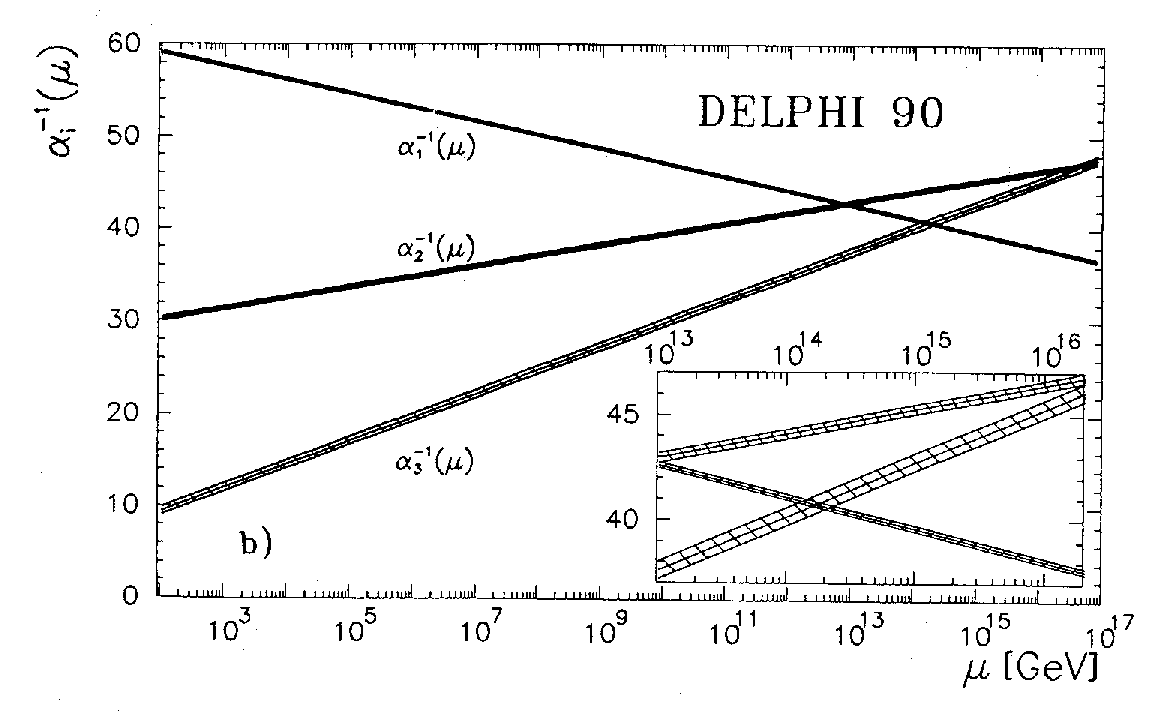
\includegraphics[width=0.49\textwidth]{figures/theory/running_couplings_SM}
      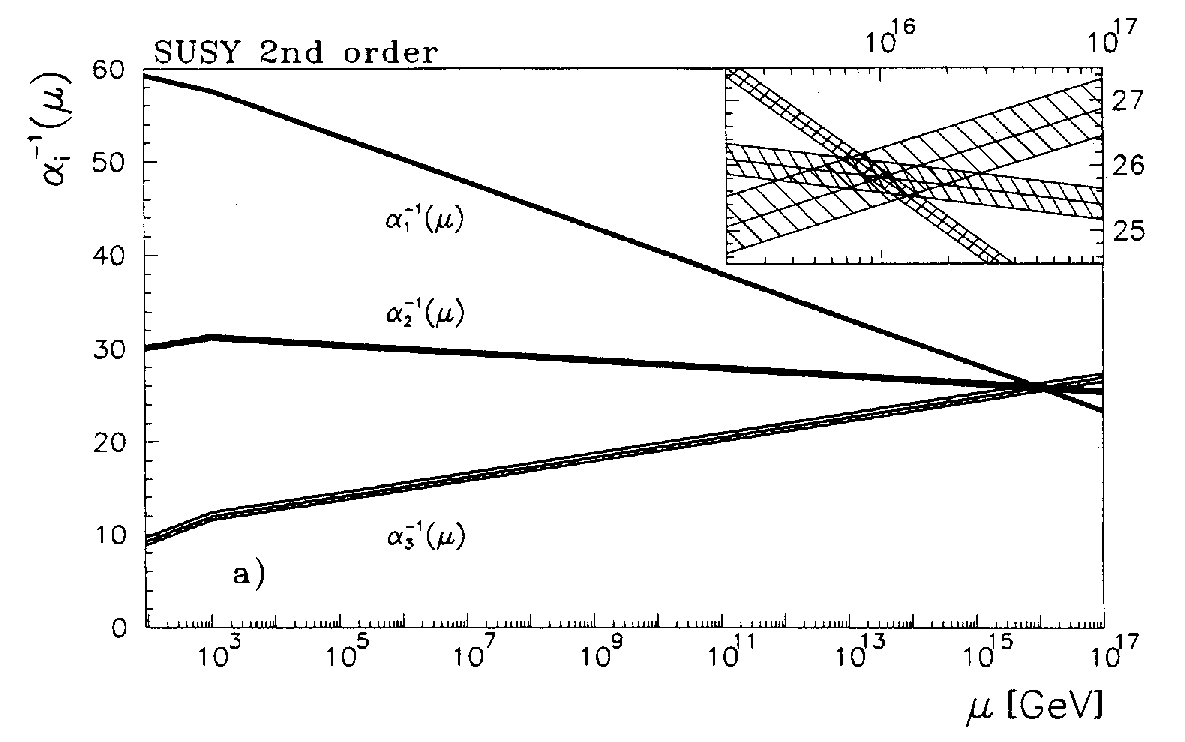
\includegraphics[width=0.49\textwidth]{figures/theory/running_couplings_MSSM}
  \caption{The running of the gauge couplings in the Standard Model (left) and in the minimal supersymmetric extension of the SM (right). Taken from~\cite{bib:Unification}.}  
  \label{fig:Unification}
\end{figure}

Besides these arguments, SUSY can also give an answer to the problem of non-visible matter in the universe.
If the conservation of the so-called R-parity is required, the lightest supersymmetric particle (LSP) is stable.
If this particle is only weakly interacting, it can serve as a good candidate to explain fully or partially the sources of the relic density. 
R-parity is a multiplicative quantum number with
\begin{align*}
P_R & =  1 &&\text{SM particles}&&\\
P_R & = -1 &&\text{SUSY particles}.&&
\end{align*}
If R-parity is conserved, only terms are allowed in the Lagrangian density, that contain an even number of supersymmetric particles.
Therefore, no single SUSY particle can decay into only SM particles and thus, the LSP is stable.



\section{The MSSM}
\label{sec:MSSM}
The supersymmetric extension of the Standard Model with a minimal particle content is called the Minimal Supersymmetric Standard Model (MSSM).
In the following section, the particle content of the MSSM is introduced.

\subsection{The particle content of the MSSM}
In $N=1$ Supersymmetry, every SM particle has exactly one supersymmetric partner particle, which leads to a doubling of the particle content in the MSSM with respect to the SM.
Additionally, there is a necessity for a second Higgs doublet.
The second doublet is needed to ensure the holomorphicity of the superpotential when also mass terms for the up-type particles shall be created.
Furthermore, the MSSM stays only free from anomalies if there is a further Higgs doublet.
This leads to the fact, that in the MSSM, there are five Higgs bosons instead of only one as in the SM.
The complete particle content of the MSSM is depicted in Tables~\ref{tab:chiral_multiplets} and~\ref{tab:vector_multiplets}.

Since in supersymmetric theories only left-handed Weyl spinors appear in the Lagrangian density, the right-handed are described as charge conjugated spinors of the left-handed spinors.

\renewcommand{\arraystretch}{1.5}
\begin{table}[!h]
\centering
\caption{Chiral supermultiplets in the MSSM}
\label{tab:chiral_multiplets}
\makebox[0.99\textwidth]{
\begin{tabular}{l|c|c|c|c}
\multicolumn{5}{c}{} \\
\toprule
                     &           &   spin 0                                     & spin $\frac{1}{2}$              & $SU(3)_C,\ SU(2)_L,\ U(1)_Y$\\ 
\midrule
   squarks/quarks    & Q         & $\left(\tilde{u}_L,\tilde{d}_L \right)$      & $\left(u_L,d_L\right)$          & $\bf{3},\ \bf{2},\ \frac{1}{3}$\\ \cline{2-5}  
                     & $\bar{u}$ & $\tilde{\bar{u}}_L = \tilde{u}_R^{\dagger} $   & $\bar{u}_L = (u_R)^c$           & $\bf{\bar{3}},\ \bf{1},\ -\frac{4}{3}$\\ \cline{2-5}  
                     & $\bar{d}$ & $\tilde{\bar{d}}_L = \tilde{d}_R^{\dagger}$    & $\bar{d}_L = (d_R)^c$           & $\bf{\bar{3}},\ \bf{1},\ \frac{2}{3}$\\ 
\midrule
   sleptons/leptons  & L         & $\left(\tilde{\nu}_{eL},\tilde{e}_L\right)$   & $\left(\nu_{eL},e_L\right)$     & $\bf{1},\ \bf{2},\ -1$\\ \cline{2-5} 
                     & $\bar{e}$ & $\tilde{\bar{e}}_L = \tilde{e}_R^{\dagger}$    & $\bar{e}_L = (e_R)^c$           & $\bf{\bar{1}},\ \bf{1},\ 2$\\ 
\midrule
   Higgs/higgsinos   & $H_u$     & $\left(H_u^+,H_u^0\right)$        & $\left(\tilde{H}_u^+,\tilde{H}_u^0\right)$ & $\bf{1},\ \bf{2},\ 1$\\ \cline{2-5}
                     & $H_d$     & $\left(H_d^0,H_d^-\right)$        & $\left(\tilde{H}_d^0,\tilde{H}_d^-\right)$ & $\bf{1},\ \bf{2},\ -1$ \\ 
\bottomrule
\multicolumn{5}{c}{} \\
\end{tabular}}
\end{table}  

\renewcommand{\arraystretch}{1.5}
\begin{table}[!h]
\centering
\caption{Vector supermultiplets in the MSSM}
\label{tab:vector_multiplets}
\makebox[0.99\textwidth]{
\begin{tabular}{l|c|c|c}
\multicolumn{4}{c}{} \\
\toprule
                      &   spin $\frac{1}{2}$                                  & spin 0                 & $SU(3)_C,\ SU(2)_L,\ U(1)_Y$\\ 
\midrule
   gluinos/gluons     & $\tilde{g}$                       & $g$                 & $\bf{8},\ \bf{1},\ 0$\\ 
\midrule
   winos/$W$-bosons   & $\tilde{W}^{\pm},\ \tilde{W}^0$  & $W^{\pm},\ W^0$     & $\bf{1},\ \bf{3},\ 0$\\
\midrule
   bino/$B$-boson       & $\tilde{B}$                      & $B$                 & $\bf{1},\ \bf{1},\ 0$ \\  
\bottomrule
\multicolumn{4}{c}{} \\
\end{tabular}}
\end{table}  



\subsection{The Lagrangian density of the MSSM}
\label{sec:Lagrange_MSSM}
In the following only the most important parts of the MSSM Lagrangian density will be described.
The reader is again referred to~\cite{bib:Drees_2004} for a complete description of the Lagrangian density.

\subsubsection*{The superpotential}
The superpotential of the MSSM contains the self interaction terms of the Higgs bosons and generates the interaction terms of the Higgs bosons with the fermions and their superpartners.
As already noted, it is very common to assume R-parity conservation.
Hence, no terms appear in the Lagrangian that would violate lepton or baryon number conservation and the lightest supersymmetric particle is stable.
Thus, all possible terms are
\begin{equation}
\label{eq:SPMSSM}
 W_{\text{MSSM}} = \mu H_u \cdot H_d - Y_u^{ij} H_u \cdot Q_L^i u_R^{c\,j} + Y_d^{ij} H_d \cdot Q_L^i d_R^{\,c\,j} + Y_e^{ij} H_d \cdot L_L^i e_R^{c\,j},
\end{equation}
with the dot product defined as in~\cite{bib:Aitchison_2005} 
\begin{equation}
 A \cdot B = \epsilon^{\alpha\beta} A_{\alpha} B_{\beta} = A_1 B_2 - A_2 B_1.
\end{equation}

\subsubsection*{The soft-breaking Lagrangian density}
Since Supersymmetry is broken, explicit SUSY breaking terms are added to the Lagrangian density.
In order not to introduce new sources of quadratic divergencies, only bilinear and trilinear terms appear in the soft-breaking Lagrangian
\begin{equation}
 \begin{split}
  - \mathcal{L}^{MSSM}_{soft} =\,& m_{H_u}^2 H_u^{\dagger} \cdot H_u +m_{H_d}^2 H_d^{\dagger} \cdot H_d + \left(B\mu\, H_u \cdot H_d + h.c.\right) \\
  & + m_{\tilde{Q}\,ij}^2 \tilde{Q}_{L\,i}^{\dagger} \cdot \tilde{Q}_{L\,j}+ m_{\tilde{u}\,ij}^2 \tilde{u}_{R\,i}^{c\,\dagger} \cdot \tilde{u}_{R\,j}^c
+ m_{\tilde{d}\,ij}^2 \tilde{d}_{R\,i}^{\,c\,\dagger} \cdot \tilde{d}_{R\,j}^{\,c}\\
& + m_{\tilde{L}\,ij}^2 \tilde{L}_{L\,i}^{\dagger} \cdot \tilde{L}_{L\,j}+ m_{\tilde{e}\,ij}^2 \tilde{e}_{R\,i}^{\,c\,\dagger} \cdot \tilde{e}_{R\,j}^{\,c}\\
& +\left(- \left( A_u Y_u \right)_{ij} H_u \cdot \tilde{Q}_{L\,i} \tilde{u}_{R\,j}^c +\left( A_d Y_d \right)_{ij} H_d \cdot \tilde{Q}_{L\,i} \tilde{d}_{R\,j}^{\,c} \right.\\
& \left. +\left( A_e Y_e \right)_{ij} H_d \cdot \tilde{L}_{L\,i} \tilde{e}_{R\,j}^{\,c} + h.c. \right)\\
& + \left(M_1 \tilde{B} \tilde{B} + M_2 \tilde{W}_a \tilde{W}_a + M_3 \tilde{g}_i \tilde{g}_i + h.c \right)
 \end{split}
\end{equation}
The first line contains mass terms for the Higgs bosons, the second and third line for the sfermions.
In the fourth and fifth line the trilinear couplings between the Higgs bosons and the sfermions appear.
Finally, the last line give rise to mass terms for the gauginos.

Because of the soft-breaking terms, the MSSM contains more than 100 free parameters.
Constraining the MSSM is thus a difficult task and usually in experimental particle physics, constrained versions of the MSSM or assumptions at the GUT scale are used to report the impact of searches on SUSY. 
In the following a short introduction of the phenomenological MSSM is given.
With its reduced parameter space, it allows to elaborate on long-lived particles in the MSSM in a much easier way.

\subsection{The phenomenological MSSM}
The phenomenological MSSM (pMSSM) imposes constraints that are reasonable in the sense to fulfil current observations and still keep the phenomenological richness of the MSSM~\cite{bib:pMSSM}.
The following assumptions are imposed (in~\cite{bib:pMSSM} more detailed information about these assumptions can be found):
\begin{itemize}
\item No new sources of CP violation,
\item No flavour changing neutral currents,
\item First and second generation universality.
\end{itemize}
These assumption reduce the number of SUSY parameters to only 19.
The remaining free parameters are the following:
\begin{itemize}
\item $\tan \beta$ (the ratio of the vacuum expectation values of the two Higgs doublets)
\item $M_A$ (the mass of the pseudo-scalar Higgs boson)  
\item $\mu$ (the Higgs mass parameter)
\item $M_1$,$M_2$,$M_3$ (bino, wino and gluino mass parameters, respectively)
\item $m_{\tilde{q}}$, $m_{\tilde{l}}$, $m_{\tilde{u}}$, $m_{\tilde{d}}$ and $m_{\tilde{e}}$ (the first and second generation mass parameters)
\item  $m_{\tilde{Q}}$, $m_{\tilde{L}}$, $m_{\tilde{t}}$, $m_{\tilde{b}}$ and $m_{\tilde{\tau}}$ (the third generation mass parameters)
\item $A_t$, $A_b$ and $A_{\tau}$ (third generation trilinear couplings).
\end{itemize}

\section{Supersymmetry breaking}
As already noted, the mechanism of supersymmetry breaking is unknown.
There exists however, several ideas how to spontaneously break supersymmetry.
All mechanism have in common that they need to happen at high energies in a hidden sector.
``Messenger'' particles are introduced which mediate the breaking to the TeV scale.
This, however, implies that supersymmetry breaking is a question of high-energy physics and one can always parametrise the breaking by the soft breaking terms introduced in Section~\ref{sec:Lagrange_MSSM}.

The most popular breaking mechanism is gravity mediated Supersymmetry breaking~\cite{FIXME} and gauge-mediated supersymmetry breaking~\cite{FIXME}.   


\chapter{Long-lived particles in the MSSM}

\begin{itemize}
\item Mechanism of long lifetimes
\end{itemize}

\section{Previous searches for long-lived charged particles}

